

\section{RESULTS}
\subsubsection{Density projection upon one dimension} % (fold)
\label{ssub:density_projection_upon_one_dimension}

%\begin{figure}[htbp]
%\centering
%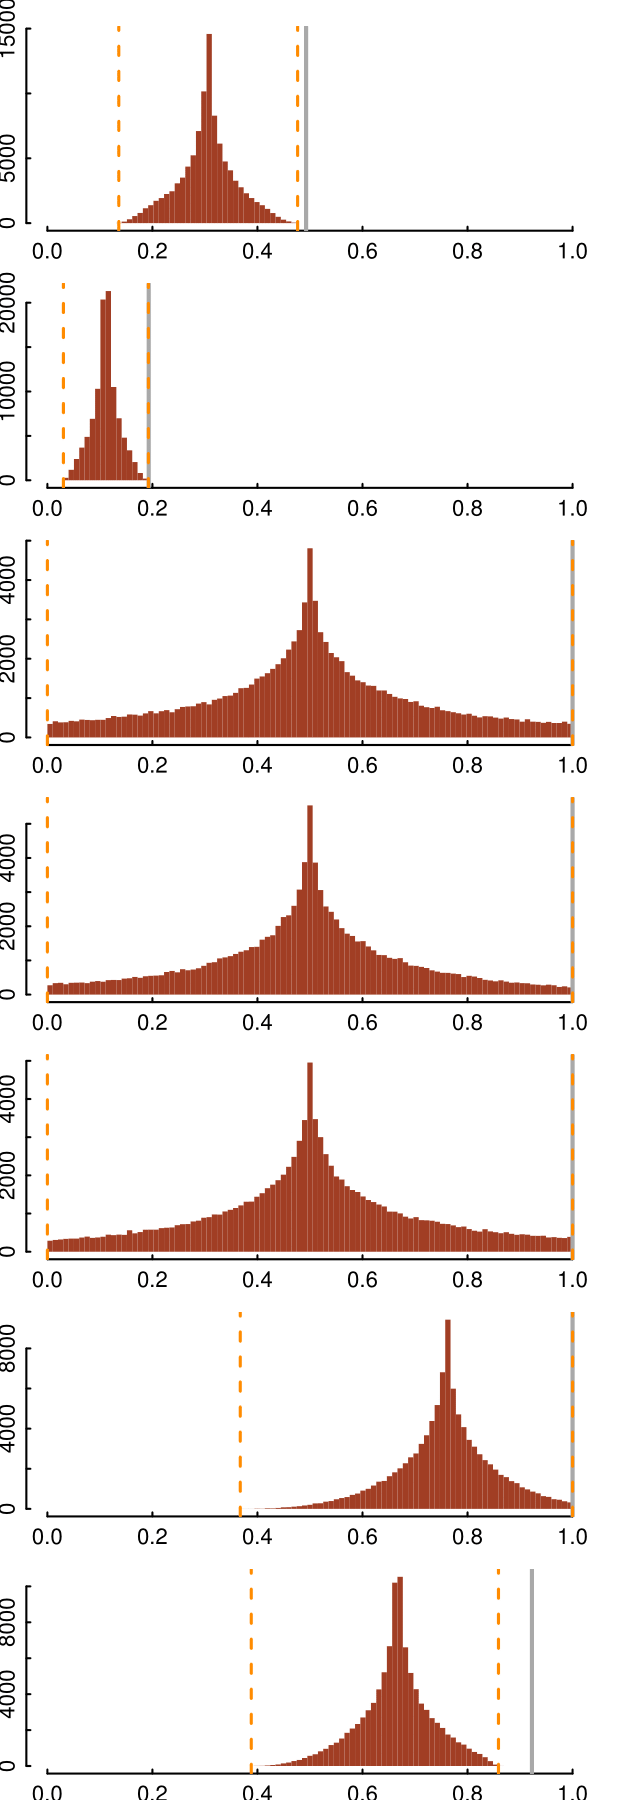
\includegraphics[width=0.5\textwidth]{sections/figs/raw_histograms.png}
%\caption{Distribution of feasible activations for [briantodo: select task percent]50\% maximal force output in the palmar direction.}
%\label{fig:raw_histograms}
%\end{figure}
Using Hit-and-Run to sample feasible activation sets, Figure \ref{fig:raw_histograms} shows the distributions of activation solutions for a palmar submaximal force resulting from [briantodo number] solutions computed with Hit-and-Run sampling. This is the first time (to our knowledge) that the internal structure of the feasible activation set has been visualized for a sub-maximal force.
Notice also that the lower and upper bounds of the activations (i.e., the dashed lines that indicate their bounding box), are uniquely uninformative of the actual density of distribution of feasible activations. Note also that the activation needed for the maximal force output (thick gray line) is very often not the mode of the activations at [briantodo select correct number]50\%[maytodo: can we set this as a variable and use throughout?] of output.
\\
This figure shows ... [briantodo]
talk about what the bounds mean with respect to the upper and lower bounds.
Talk about the function of each muscle, with respect to the moment arm matrix and the relevant cell of the A matrix.

The density integrals perpendicular to each muscle are provably unimodal due to the convexity [maytodo cite or add supporting evidence], and therefore it would be inadvisable to fit a normal distribution as the probability density function.
% subsubsection density_projection_upon_one_dimension (end)

\subsection{Activation spaces for increasing force} % (fold)
\label{sub:activation_spaces_for_increasing_force}
For maximal force into any direction, there is a unique activation vector satisfiying all constraint. The maximal force into palmar direction is given by ????? and its unique activation vector ????. [briantodo insert values]
In Figure \ref{fig:XY_progression} we give the distributions of the activations for increasing force, starting with $10\%$ of the maximal force, increasing in $10\%$ steps until maximal force is reached.

[1. briantodo generate pdfs as separate pages]
[briantodo write about how they are skewed, constrained, etc. Produce stats for each of the histograms and superimpose the data temporarily so you can write about it]

The solution polytope converges as the difficulty of the task increases; the rate of convergence is different across muscles. For some muscles (such as X and Y) the convergence only occurs in the last [briantodo insert maximal feasible palmar force * 0.90], while others converge earlier-in lower forces of maximal (X and Y are examples of this)[briantodo fill out these descriptive statistics].

It is imperative to keep in mind that every histogram (regardless of its convergence) is composed of the distribution of all 10,000 points; when the distribution is compressed, the relative percentage of the bars will increase, as we made break width ($\Delta x$) remain constant to 2\% of maximal contraction. [briantodo cite http://library.msri.org/books/Book31/files/ball.pdf]

The peaks seen in these figures refers to the perpendicular slice that has the largest area. %the highest number of points, and therefore has the highest volume (relative to the other parts).

\begin{figure}[htbp]
\centering
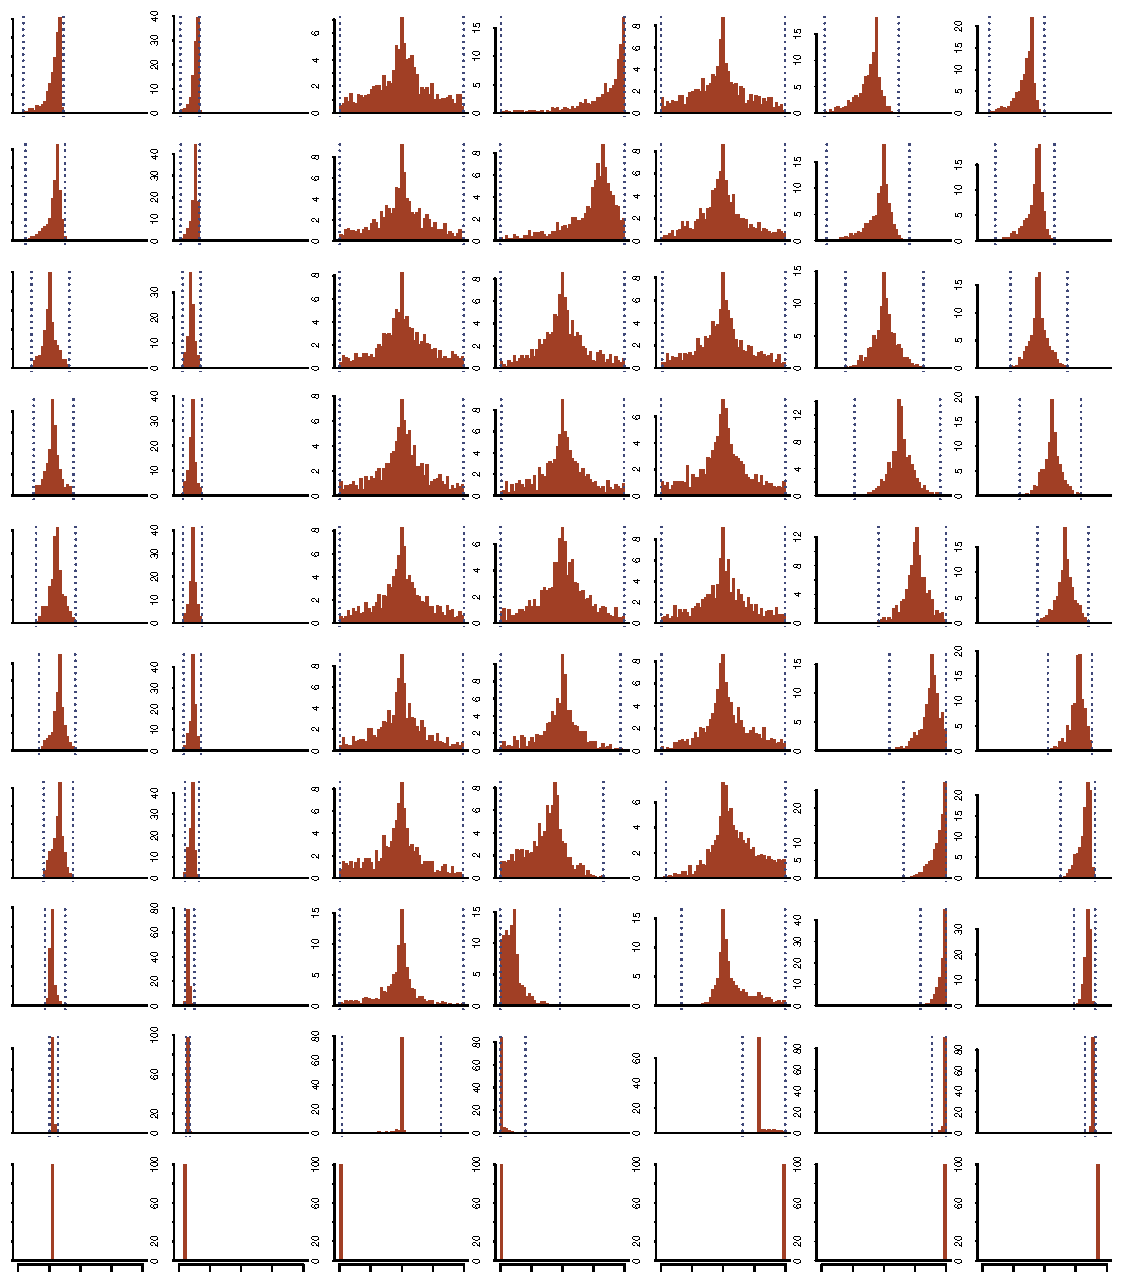
\includegraphics[width=\textwidth]{figs/Z_alphaProgression1430924065026.pdf}
\caption{Distribution of activations in the palmar direction and changing force. Each row of histograms uses a hit-and-run set. The height of each bar visualizes the percentage of 10,000 solutions found within a given 0.02 span of activation; the shape is more meaningful than the magnitude of the y axis, as we expect convergence (and therefore peak increase within few bins) towards maximal contractions. We computed the upper and lower bounds of activation for each muscle (vertical dotted lines).}
\label{fig:Z_progression}
\end{figure}
% subsection activation_spaces_for_increasing_force (end)


To maintain realtime interactivity of the plot, we used only the first 1000 points collected for each task, from 10\% to 100\%.
\label{sub:parallel_coordinates}

\begin{figure}[htbp]
\centering
\includegraphics[width=\textwidth]{figs/parcoord_alpha50.pdf}
\caption{This figure is a snapshot of the interactive platform for visualizing all solutions. This parallel coordinates plot visualizes, where each feasible activation set is strewn across each dimension's axis as a line. While alpha could be set to view all tasks, we set alpha to a palmar force of 50\% of the computed maximal feasible force in this direction. Here we show 1000 points accrued from Hit and Run on a task of $\$alpha=0.5$.}
\label{fig:parcoord_full}
\end{figure}

\begin{figure}[htbp]
\centering
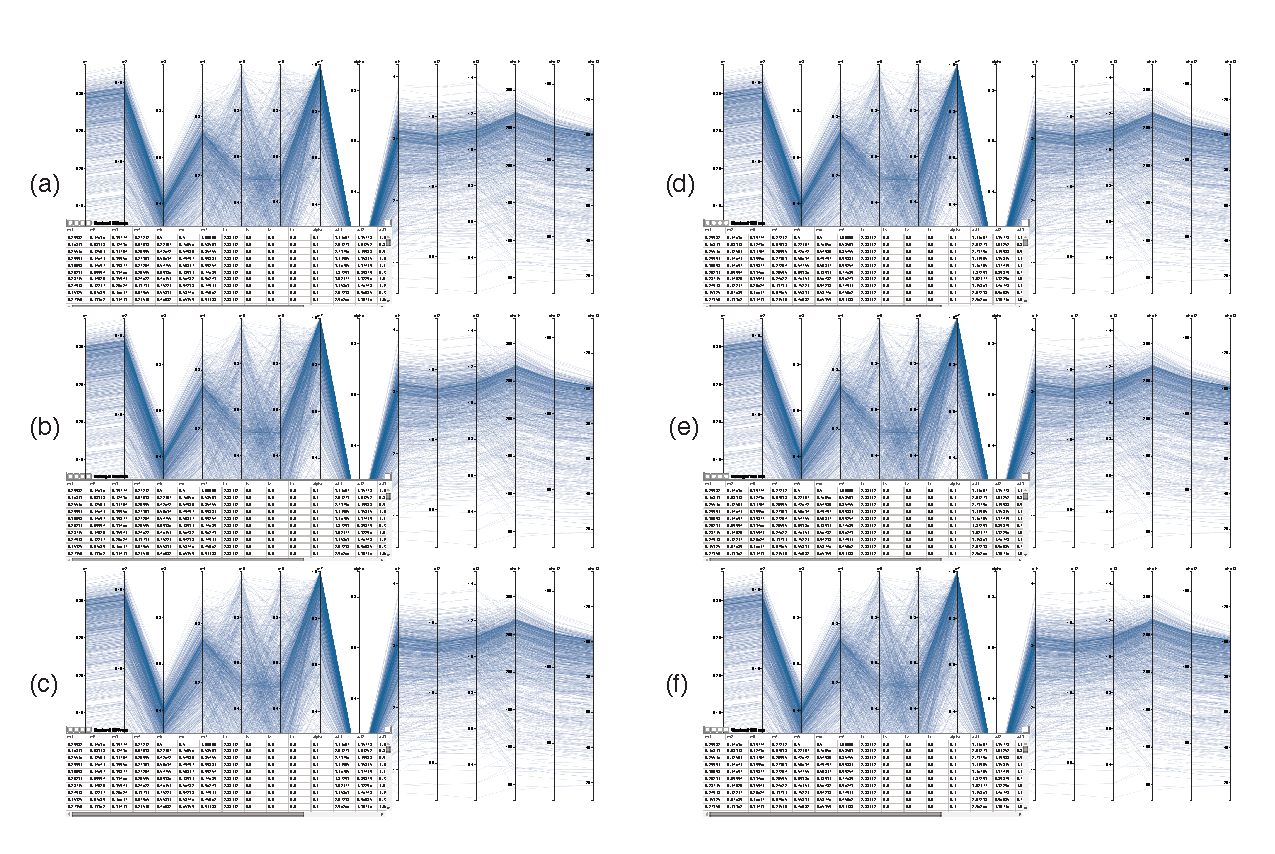
\includegraphics[width=\textwidth]{figs/parcoords.pdf}
\caption{These snapshots show the use of the interactive parallel coordinate visualization of solutions across the activation space. For the task set to 50\% of maximal in the palmar direction, we show the
(a) remaining 166 solutions when PI $<$ 60\% 
(b) remaining 57 solutions when DI $<$ 260\%, and the
(c) remaining 57 solutions when we constrain PI $<$ 60\% and DI $<$ 260\%. We also show the
(d) remaining 502 solutions when we select the lower 50\% of l1 costs,
(e) remaining 498 solutions when we select the lower 50\% of l2w costs, and the
(f) remaining 220 solutions when we select the lower 50\% across all cost functions in Table \ref{cost_function_tabls} }
\label{fig:parcoords}
\end{figure}

discuss what happens when you bring each of those muscles down, using the R produced stats.
talk about how when you add X as a constraint, most of the solutions are distributed across the other muscles between X and X. Say which ones go up, which go down- which ones become clustered and which ones lose their peak/spike.

% subsection parallel_coordinates (end)